\chapter{Continuous tempering}\label{ch:continuous-tempering}

In Chapter \ref{ch:approximate-inference} we introduced simulated tempering as an approach for dealing with two key issues with \ac{MCMC} methods: improving exploration of multi-modal distributions and allowing estimation of the normalising constants of target distributions, which is often an important quantity for model comparison.

Although \ac{HMC} is able to efficiently explore contiguous regions of high probability density in a target distribution, as with most \ac{MCMC} methods using local moves it struggles to move between isolated modes in multimodal target distributions \citep{neal2011mcmc}. Tempering methods \citep{swendsen1986replica,geyer1991markov,marinari1992simulated} which augment the state space with an temperature variable are often used to improve exploration in multimodal distributions. As the temperature variable is typically discrete however it cannot be included in \ac{HMC} updates.

In this Chapter we present an alternative \emph{continuous tempering} approach which instead augments the state with a continuous temperature variable. This allows use of \ac{HMC} to jointly update both the temperature and original state, making the method simple to use with existing \ac{HMC} implementations. The proposed approach both improves exploration of multimodal densities and also provides estimates of the typically unknown normalising constant of the target density, which is often an important inferential quantity in its own right for model comparison \citep{gelman1998simulating}.

The work described in this chapter have previously appeared in the published conference paper
\begin{itemize}
 \item Continuously tempered Hamiltonian Monte Carlo. Matthew M. Graham and Amos J. Storkey. \emph{Proceedings of the 33rd Conference on Uncertainty in Artificial Intelligence}, 2017.
\end{itemize}
I was the primary author of that publication and resposible for the novel contributions made in the paper, as well as performing and analysing the numerical experiments described in the paper, which are reproduced in this chapter in Section \ref{sec:ct-experiments}.

\section{HMC in multimodal distributions}

The energy conservation property which makes Hamiltonian dynamics a desirable proposal generating mechanism for a \ac{MCMC} method also however suggests that standard \ac{HMC} updates are unlikely to move between isolated modes in a target distribution. The Hamiltonian is approximately conserved over a trajectory therefore $\phi(\vct{x}') - \phi(\vct{x}) \approx \tau(\vct{p}) - \tau(\vct{p}')$. Typically a quadratic kinetic energy  $\tau(\vct{p}) = \vct{p}\tr\mtx{M}^{-1}\vct{p} \,/\,2$ is used corresponding to a Gaussian marginal density on the momentum. As this kinetic energy is bounded below by zero, the maximum change in potential energy over a trajectory is approximately equal to the initial kinetic energy. 

At equilibrium the momenta will have a Gaussian distribution and so the kinetic energy a $\chi^2$ distribution with mean $\nicefrac{D}{2}$ and variance $D$ \citep{neal2011mcmc,betancourt2013general}. If potential energy barriers significantly larger than $\sim D$ separate regions of the configuration state space the \ac{HMC} updates are unlikely to move across the barriers meaning impractically long sampling runs will be needed for effective ergodicity.

\section{Thermodynamic methods}

An alternative is \ac{PT} \citep{swendsen1986replica,geyer1991markov,earl2005parallel}, where multiple Markov chains on the target state are run in parallel, with the $n$\textsuperscript{th} chain having an associated inverse temperature $\beta_n$ defined as in \eqref{eq:finite-inv-temp-schedule}. \ac{MCMC} updates are performed on each chain which leave a distribution with unnormalised density $\pi(\vct{x} \gvn \beta_n)$ invariant. Interleaved with these updates, exchanges of the states of the chains at adjacent inverse temperatures $(\beta_n,\,\beta_{n+1})$ are proposed in a Metropolis--Hastings step. Parallel tempering sidesteps the issue with mixing between inverse temperatures in \ac{ST} by keeping the inverse temperatures for the chains fixed, at a cost of a significantly increased state size.

\emph{Tempered transitions} \citep{neal1996sampling} uses a different approach, deterministically altering the inverse temperature rather than including it as part of the Markov chain state. Again an ordered set of inverse temperatures are specified as in \eqref{eq:finite-inv-temp-schedule}. For each inverse temperature $\beta_n : n > 0$ a pair of transition operators $\hat{\transop}_n$, $\check{\transop}_n$ are defined which satisfy a reversibility condition $\hat{\transop}_n[\vct{x}' \gvn \vct{x}] \pi(\vct{x} \gvn \beta_n) = \check{\transop}_n[ \vct{x} \gvn \vct{x}'] \pi(\vct{x}' \gvn \beta_n)$ (if $\hat{\transop}_n = \check{\transop}_n$ this is just detailed balance). The transition operators associated with lower inverse-temperatures will typically be able to make larger moves in the state space. 

These transition operators are applied to the current state in a fixed sequence $\hat{\transop}_1 \dots \hat{\transop}_N  \check{\transop}_N \dots \check{\transop}_1$ to generate a chain of intermediate states, with the idea that in the initial `heating' stage $\hat{\transop}_1 \dots \hat{\transop}_N$ the state will be roughly distributed after each transition according to the target distribution at an increasing series of temperatures before being `cooled' back down with the transitions $\check{\transop}_N \dots \check{\transop}_1$ so that the final state is approximately distributed according to the target (with $\beta_0 = 1$) again. The overall transition from the initial state to the final state in the chain is then accepted or rejected in a Metropolis--Hastings step. A \ac{HMC} specific variation of this idea in which the tempering is applied within a simulated trajectory by scaling the momenta in a deterministic sequence has also been proposed \citep{neal2011mcmc}.

\ac{AIS} \citep{neal2001annealed} is another thermodynamic ensemble method, closely related to \emph{Tempered Transitions} \citep{neal1996sampling} and often the `go-to' method for normalising constant estimation in the machine learning literature e.g \citep{salakhutdinov2008quantitative,wu2016quantitative}. In \ac{AIS} an ordered set of inverse temperatures are defined as in \eqref{eq:finite-inv-temp-schedule} and a corresponding series of transition operators $\lbrace \transop_n \rbrace_{n=1}^{N-1}$. Each $\transop_n$ leaves a distribution with unnormalised density $\pi(\vct{x}\gvn\beta_n)$ invariant. Assuming the base distribution corresponding to $\beta_0 = 0$ can be sampled from independently, an independent state $\vct{x}^{(0)}$ from this distribution is generated and then the transition operators applied in a fixed sequence $\transop_{1} \dots \transop_{N-1}$ to generate a chain of intermediate states $\lbrace \vct{x}^{(n)} \rbrace_{n=1}^{N-1}$. The product of ratios
\begin{equation}\label{eq:ais-weights}
  r = \prod_{n=0}^{N-1} \lpa \pi\lpa\vct{x}^{(n)}\gvn\beta_{n+1}\rpa / \pi\lpa\vct{x}^{(n)}\gvn\beta_n\rpa \rpa
\end{equation}
is an importance weight for the final state $\vct{x}^{(N-1)}$ with respect to the target distribution \eqref{eq:target-density} and also an unbiased estimator for $\normconst$. By simulating multiple independent runs of this process, a set of importance weighted samples can be computed to estimate expectations with respect to the target \eqref{eq:target-density} and the weights $r$ used to unbiasedly estimate $\normconst$. Due to Jensen's inequality the unbiased estimate of $\normconst$ corresponds to a stochastic lower bound on $\log \normconst$ \citep{grosse2015sandwiching}.

In cases where an exact sample from the target distribution can be generated, running reversed \ac{AIS} from the target to base distribution allow calculating an unbiased estimate of $\normconst^{-1}$ and so a stochastic upper bound on $\log \normconst$ \citep{grosse2015sandwiching}. This combination of stochastically lower bounding $\log \normconst$ by forward \ac{AIS} runs and stochastically upper bounding by reverse \ac{AIS} runs is termed \emph{bidirectional Monte Carlo}.

The application of \ac{HMC} updates for the transition operators $\transop_n$ in \ac{AIS} was explored in \citep{sohl2012hamiltonian} and termed \emph{Hamiltonian \ac{AIS}}. The authors suggest using many transitions composed of a single leapfrog step and partial momentum resampling can be preferable to a smaller number of transitions using multiple leapfrog steps and full momentum resampling. 

\section{Continuous tempering}

In all three of \ac{AIS}, \ac{PT} and \ac{ST} the choice of the discrete inverse temperature schedule \eqref{eq:finite-inv-temp-schedule} is key to getting the methods to perform well in complex high dimensional distributions \citep{neal1996sampling,behrens2012tuning,betancourt2014adiabatic}. To get reasonable performance it may be necessary to do preliminary pilot runs to guide the number of inverse temperatures and spacing between them to use, adding to the computational burden and difficulty of using these methods in a black-box fashion. A natural question is therefore whether it is possible to use a continuously varying inverse temperature variable. % to side-step the need to choose a set of values. 

\emph{Path sampling} \citep{gelman1998simulating} proposes this approach, defining a general \emph{path} as a function parametrised by $\beta$ which continuously maps between the target density $\exp\lpa-\phi(\vct{x})\rpa / \normconst$  at $\beta=1$ and a base density $\exp\lpa-\psi(\vct{x})\rpa$ at $\beta = 0$, with the geometric bridge in \eqref{eq:geometric-bridge} a particular example. A joint target $\pden{\rvct{x},\upbeta}(\vct{x},\beta) \propto \pi(\vct{x}\gvn\beta) \,\rho(\beta)$ is defined with $\rho(\beta)$ a chosen prior on the inverse temperature variable analogous to the weights $\lbrace w_n \rbrace_{n=0}^N$ in simulated tempering. In \citep{gelman1998simulating} it is proposed to construct a Markov chain leaving the joint density invariant by alternating updates of $\rvct{x}\gvn\upbeta$ and $\upbeta\gvn\rvct{x}$. Samples from the joint system can be used to estimate $\normconst$ via the \emph{thermodynamic integration} identity
\begin{equation}\label{thermodynamic-integration}
\log \normconst = 
\int_0^1 \hspace{-0.5em} \int_{\set{X}}
  \frac{\pden{\rvct{x},\upbeta}(\vct{x},\beta)}{\pden{\upbeta}(\beta)}\,
  \pd{\log\pi(\vct{x}\gvn\beta)}{\beta}
\,\dr\vct{x}\,\dr\beta.
\end{equation}

\emph{Adiabatic Monte Carlo} \citep{betancourt2014adiabatic} also proposes using a continuously varying inverse temperature variable, here specifically in the context of \ac{HMC}. The original Hamiltonian system $(\rvct{x},\,\rvct{p})$ is further augmented with a continuous inverse temperature coordinate $\upbeta \in [0,\,1]$. %Utilising the differential geometric theory of contact manifolds, 
A \emph{contact Hamiltonian} is defined on the augmented system, 
\begin{equation}\label{eq:contact-hamiltonian}
\begin{split}
  \hamiltonian_c(\vct{x},\,\vct{p},\,\beta) = \beta \phi(\vct{x}) &+ ( 1 - \beta ) \psi(\vct{x}) 
  + \frac{1}{2}\vct{p}\tr\mtx{M}^{-1}\vct{p} \\
  &+ \log \partfunc(\beta) + \hamiltonian_0
\end{split}
\end{equation}
this defining a corresponding \emph{contact Hamiltonian flow}, 
\begin{equation}\label{eq:contact-hamiltonian-flow}
  \td{\vct{x}}{t} = \pd{\hamiltonian_c}{\vct{p}}\tr\kern-3pt,\,
  \td{\vct{p}}{t} = \pd{\hamiltonian_c}{\beta} \vct{p} -\pd{\hamiltonian_c}{\vct{x}}\tr\kern-3pt,\,
  \td{\beta}{t} = \hamiltonian_c - \pd{\hamiltonian_c}{\vct{p}}\vct{p}.
\end{equation}
The contact Hamiltonian flow restricted to the zero level-set of the contact Hamiltonian (which the initial state can always be arranged to lie in by appropriately choosing the arbitrary constant $\hamiltonian_0$) generates trajectories which exactly conserve the contact Hamiltonian and extended state space volume element, and correspond to the thermodynamical concept of a reversible adiabatic process. 

For a quadratic kinetic energy, $\td{\beta}{t}$ is always non-positive and so forward simulation of the contact Hamiltonian flow generates non-increasing trajectories in $\beta$ (and backwards simulation generates non-decreasing trajectories in $\beta$). In the ideal case this allows the inverse temperature range $[0,\,1]$ to be coherently traversed without the random-walk exploration inherent to simulated tempering.

Simulating the contact Hamiltonian flow is non-trivial in practice however: the contact Hamiltonian \eqref{eq:contact-hamiltonian} depends on the log partition function $\log \partfunc(\beta)$, the partial derivatives of which require computing expectations with respect to $\pi(\vct{x}\gvn\beta)$ which for most problems is intractable to do exactly. Moreover the contact flow can encounter meta-stabilities whereby $\td{\beta}{t}$ becomes zero and the flow halts at an intermediate $\beta$ meaning the flow no longer defines a bijection between $\beta=0$ and $\beta=1$. This can be ameliorated by regular resampling of the momenta however this potentially increases random-walk behaviour of the overall dynamic.

An alternative \emph{extended Hamiltonian approach} for simulating a system with a continuously varying inverse temperature was proposed recently in the statistical physics literature \citep{gobbo2015extended}. The inverse temperature of the system is indirectly set via an auxiliary variable, which we will term a \emph{temperature control variable} $\rvar{u} \in \reals$. This control variable is mapped to an interval $[s,\,1]$, $0 < s < 1$ via a smooth piecewise defined function $\beta : \reals \to [s,\,1]$, with the conditions that for a pair of thresholds $(\theta_1,\,\theta_2)$ with $0 < \theta_1 < \theta_2$, $\beta(u) = 1 ~\forall~ |u| \leq \theta_1$, $\beta(u) = s ~\forall~ |u| \geq \theta_2$ and $s < \beta(u) < 1 ~\forall~ \theta_1 < |u| < \theta_2$.

Unlike Adiabatic Monte Carlo, an additional momentum variable $\rvar{v}$ corresponding to $\rvar{u}$ is also introduced. Although seemingly a minor difference this simplifies the implementation of the approach significantly as the system retains a symplectic structure and can continue to be viewed within the usual Hamiltonian dynamics framework. An \emph{extended Hamiltonian} is defined on the augmented system
\begin{equation}\label{eq:extended-hamiltonian-gobbo-leimkuhler}
  \extended{\hamiltonian}(\vct{x},\,u,\,\vct{p},\,v) = 
  \beta(u) \phi(\vct{x}) + \omega(u) + \frac{1}{2} \vct{p}\tr\mtx{M}^{-1}\vct{p} + \frac{v^2}{2m}
\end{equation}
where $\omega$ is a `confining potential' on $u$ and $m$ is the mass (marginal variance) associated with $\rvar{v}$. This extended Hamiltonian is separable with respect to the extended configuration $(\rvct{x},\,\rvar{u})$ and extended momentum $(\rvct{p},\,\rvar{v})$ and so can be efficiently simulated using a standard leapfrog integrator. In \cite{gobbo2015extended} the extended Hamiltonian dynamics are integrated using a Langevin scheme without Metropolis adjustment and shown to improve mixing in several molecular dynamics problems. 

Due to the condition $\beta(u) = 1 ~\forall~ |u| < \theta_1$, the set of sampled configuration states $\rvct{x}$ which have associated $|\rvar{u}| < \theta_1$ will (assuming the dynamic is ergodic and Metropolis adjustment were used) asymptotically converge in distribution to the target, and so can be used to estimate expectations without any importance re-weighting. The $\beta$ function is required to be bounded below by a $s > 0$ in \citep{gobbo2015extended} due to the base density being bridged to being an improper uniform density on $\set{X}$. The partition function $\partfunc(\beta) \to \infty$ as $\beta \to  0$ in this case, which would imply an infinite density for regions in the extended state space where $\beta(\rvar{u}) = 0$. Even with a non-zero lower bound on $\beta$, the large variations in $\partfunc\lpa\beta(\rvar{u})\rpa$  across different $\rvar{u}$ values can lead to the dynamic poorly exploring the $\rvar{u}$ dimension. 

In \citep{gobbo2015extended} this issue is tackled by introducing an adaptive history-dependent biasing potential on $\rvar{u}$ to try to achieve a flat density across a bounded interval $|\rvar{u}| < \theta_2$, using for example metadynamics \citep{laio2002escaping}. The resulting non-Markovian updates bias the invariant distribution of the target state however this can be accounted for either by a re-weighting scheme \citep{bonomi2009reconstructing}, or using a vanishing adaptation.

\section{Proposed method}\label{sec:proposed-approach}

As in \citep{gobbo2015extended} we define an extended Hamiltonian on an augmented state $(\rvct{x},\,\rvar{u})$ with associated momenta $(\rvct{p},\,\rvar{v})$,
\begin{align}\nonumber
  \extended{\hamiltonian}(\vct{x},u,\vct{p},v) =&
  \beta(u) \lpa \phi(\vct{x}) + \log\zeta\rpa + 
  \lpa 1 - \beta(u) \rpa \psi(\vct{x}) \\ \label{eq:extended-hamiltonian}
  &- \log\left|\pd{\beta}{u}\right| +
  \frac{1}{2} \vct{p}\tr\mtx{M}^{-1}\vct{p} + \frac{v^2}{2m}.
\end{align}

As with the approach of \citep{gobbo2015extended}, this Hamiltonian is separable and the corresponding dynamic can be efficiently simulated with a leapfrog integrator. The reversible and volume-preserving simulated dynamic can then be used as a proposal generating mechanism on the joint space $(\rvct{x},\,\rvar{u},\,\rvct{p},\,\rvar{v})$ for a Metropolis--Hastings step as in standard \ac{HMC}. We will term this approach of running \ac{HMC} in the extended joint space \emph{joint continuous tempering}.

In contrast to \citep{gobbo2015extended} we propose to use a smooth monotonically increasing map $\beta : \reals \to [0, 1]$ as the inverse temperature function, with our default choice in all experiments being the logistic sigmoid $\beta(u) = \lpa 1 + \exp(-u)\rpa^{-1}$.

As previously $\psi$ is the negative logarithm of a simple \emph{normalised} base density, which (as we will motivate in the next section) we will usually choose to be an approximation to the target density \eqref{eq:target-density}. Similarly the $\log\zeta$ term will be chosen to be an approximation to $\log \normconst$.

We can marginalise out the momenta from the joint distribution defined by this Hamiltonian, giving a joint density
\begin{equation}\label{eq:x-u-joint-density}
\begin{split}
\pden{\rvct{x},\rvar{u}}(\vct{x},u) \propto \left|\pd{\beta}{u}\right| 
\exp\Big(&
  -\beta(u)\lpa \phi(\vct{x}) + \log\zeta\rpa\\[-1mm]
  &- \lpa 1 - \beta(u)\rpa\psi(\vct{x})
\Big).
\end{split}
\end{equation}
If we define a variable $\upbeta = \beta(\rvar{u})$ and use the change of variables formula for a density, we further have that
\begin{equation}\label{eq:x-beta-joint-density}
\pden{\rvct{x},\upbeta}(\vct{x},\beta) \propto \frac{1}{\zeta^\beta}
\exp \lpa
  -\beta \phi(\vct{x}) - ( 1 - \beta)\psi(\vct{x})
\rpa
\end{equation}

The bijectivity between $\rvar{u}$ and $\upbeta$ is useful as although if simulating a Hamiltonian dynamic we will generally wish to work with $\rvar{u}$ as it is unbounded, the conditional density on $\upbeta$ given $\rvct{x}$ has a tractable normalised form
\begin{equation}\label{eq:beta-gvn-x-density}
\pden{\upbeta|\rvct{x}}(\beta \gvn\vct{x}) = 
\frac{\exp\lpa - \beta\Delta(\vct{x})\rpa\Delta(\vct{x})}{1 - \exp\lpa-\Delta(\vct{x})\rpa},
\end{equation}
with $\Delta(\vct{x}) = \phi(\vct{x}) + \log\zeta - \psi(\vct{x})$. This corresponds to an exponential distribution with rate parameter $\Delta(\vct{x})$ truncated to $[0, 1]$. As an alternative to the joint updates, another option is therefore to form a Markov chain which leaves \eqref{eq:x-beta-joint-density} invariant by alternating independently sampling $\upbeta$ from its conditional given $\rvct{x}$ and performing a transition which leaves the conditional on $\rvct{x}$ given $\upbeta$ invariant, similar to the suggested approach in \citep{gelman1998simulating}. We will term this Gibbs sampling type procedure as \emph{Gibbs continuous tempering}.

Further we can use \eqref{eq:beta-gvn-x-density} to write the marginal density $\pden{\upbeta}$
\begin{equation}\label{eq:ct-beta-marginal}
\pden{\upbeta}(\beta) =
\expc{\frac{\exp\lpa - \beta\Delta(\rvct{x})\rpa\Delta(\rvct{x})}{1 - \exp\lpa-\Delta(\rvct{x})\rpa}}.
\end{equation}

By integrating the joint \eqref{eq:x-beta-joint-density} over $\set{X}$ we also have that
\begin{equation}\label{eq:beta-marginal-0-1}
\begin{split}
\pden{\upbeta}(\beta) = \frac{1}{C\zeta^\beta} \int_{\set{X}} 
  \pi(\vct{x}\gvn\beta)
\,\dr\vct{x} =
\frac{\partfunc(\beta)}{C\zeta^\beta}\\
\Rightarrow ~
\pden{\upbeta}(0) = \frac{1}{C}
,~
\pden{\upbeta}(1) = \frac{\normconst}{C \zeta},
\end{split}
\end{equation}
for an unknown normalising constant $C$ of the joint, and so for \ac{MCMC} samples $\lbr \vct{x}^{(s)},\,\beta^{(s)}\rbr_{s=1}^S$ from the joint \eqref{eq:x-beta-joint-density}
\begin{equation}\label{eq:ct-norm-const-estimator}
\normconst = \frac{\pden{\upbeta}(1)}{\pden{\upbeta}(0)} \zeta = 
\lim_{S\to\infty} \frac
{\sum_{s=1}^S\lpa w_1\lpa \vct{x}^{(s)}\rpa\rpa}
{\sum_{s=1}^S\lpa w_0\lpa \vct{x}^{(s)}\rpa\rpa}
\zeta,
\end{equation}
\begin{equation*}
\textrm{with }
w_0(\vct{x}) = \frac{\Delta(\vct{x})}{1 - \exp\lpa-\Delta(\vct{x})\rpa},~
w_1(\vct{x}) = \frac{\Delta(\vct{x})}{\exp\lpa\Delta(\vct{x})\rpa - 1}.
\end{equation*}
This can be seen to be a continuous analogue of the \emph{Rao-Blackwellised} estimator \eqref{eq:rao-blackwell-tempered-sampling} used in \cite{carlson2016partition}. Similarly we can calculate consistent estimates of expectations with respect to the target density $\pden{\rvct{x}|\upbeta}(\vct{x}\gvn 1) = \exp\lpa-\phi(\vct{x})\rpa / Z$ as importance weighted sums
\begin{align}\label{eq:ct-target-expc-estimator}
\expc{f(\rvct{x})\gvn\upbeta=1} &=
\frac{
  \int_{\set{X}} 
    f(\vct{x})\, \pden{\upbeta|\rvct{x}}(1 \gvn \vct{x}) \, \pden{\rvct{x}}(\vct{x})
  \,\dr\vct{x}
}{
  \int_{\set{X}} 
    \pden{\upbeta|\rvct{x}}(1 \gvn \vct{x}) \, \pden{\rvct{x}}(\vct{x})
  \,\dr\vct{x}
} 
\nonumber\\
&\approx
\frac
{\sum_{s=1}^S \lpa w_1\lpa \vct{x}^{(s)}\rpa f\lpa\vct{x}^{(s)}\rpa\rpa}
{\sum_{s=1}^S\lpa w_1\lpa \vct{x}^{(s)}\rpa \rpa}.
\end{align}
We can also estimate expectations with respect to the base density $\pden{\rvct{x}|\upbeta}(\vct{x}\gvn 0) = \exp\lpa-\psi(\vct{x})\rpa$ using
\begin{equation}\label{eq:ct-base-expc-estimator}
\expc{f(\rvct{x})\gvn\upbeta=0}
\approx
\frac
{\sum_{s=1}^S \lpa w_0\lpa \vct{x}^{(s)}\rpa f\lpa\vct{x}^{(s)}\rpa\rpa}
{\sum_{s=1}^S\lpa w_0\lpa \vct{x}^{(s)}\rpa \rpa}.
\end{equation}
Often the base density will have known moments (e.g. mean and covariance of a Gaussian base density) which can be compared to the estimates calculated using \eqref{eq:ct-base-expc-estimator} to check for convergence problems. Convergence of the estimates to the true moments is not a sufficient condition for convergence of the chain to the target joint density \eqref{eq:x-beta-joint-density} but is necessary.

\section{Bounding the inverse temperature marginal density}

We have a joint density on $(\rvct{x},\,\upbeta)$
\begin{equation}
\pden{\rvct{x},\upbeta}(\vct{x},\beta) =
\frac{1}{C} \exp\lpa -\beta\phi(\vct{x}) -\beta\log\zeta -(1-\beta)\psi(\vct{x})\rpa.
\label{eq:x-beta-joint-density-app}
\end{equation}
The resulting marginal density on $\upbeta$ is
\begin{equation}\label{eq:beta-marginal-density}
\pden{\upbeta}(\beta) = \int_{\set{X}} \pden{\rvct{x},\upbeta}(\vct{x},\beta) \,\dr\vct{x}
= \frac{1}{C\zeta^\beta} \int_{\set{X}} \exp\lpa -\beta\phi(\vct{x}) -(1-\beta)\psi(\vct{x})\rpa\,\dr\vct{x}.
\end{equation}
To derive an upper-bound on $\pden{\upbeta}(\beta)$ we use H\"older's inequality
\begin{equation}\label{eq:holders-inequality}
  \int_{\set{X}} g(\vct{x}) h(\vct{x}) \,\dr\vct{x} \leq 
  \lpa \int_{\set{X}} |g(\vct{x})|^{\frac{1}{a}} \,\dr\vct{x} \rpa^{a}
  \lpa \int_{\set{X}} |h(\vct{x})|^{\frac{1}{1-a}} \,\dr\vct{x} \rpa^{1-a}
\end{equation}
where $a \in [0,\,1]$ and $g$ and $h$ are measurable functions. We also use the definitions 
\begin{equation}\label{eq:target-and-based-norm-consts}
  \int_\set{X} \exp\lpa-\phi(\vct{x})\rpa\,\dr\vct{x} = Z
  \quad\text{and}\quad
  \int_\set{X} \exp\lpa-\psi(\vct{x})\rpa\,\dr\vct{x} = 1.
\end{equation}
From \eqref{eq:beta-marginal-density} we have that
\begin{equation}
  \pden{\upbeta}(\beta)
  =
  \frac{1}{C\zeta^{\beta}} 
  \int_\set{X} 
    \lpa \exp\lpa-\phi(\vct{x}) \rpa^{\beta}\rpa \lpa \exp\lpa-\psi(\vct{x})\rpa^{1 - \beta}\rpa
  \,\dr\vct{x}.
\end{equation}
Applying H\"older's inequality \eqref{eq:holders-inequality} with $g(\vct{x}) = \exp\lpa-\phi(\vct{x})\rpa^{\beta}$, $h(\vct{x}) = \exp\lpa-\psi(\vct{x})\rpa^{1-\beta}$ and $a = \beta$
\begin{align}
  \pden{\upbeta}(\beta)
  &\leq
  \frac{1}{C\zeta^{\beta}} 
  \lpa
  \int_\set{X} 
    \left| \exp\lpa-\phi(\vct{x}) \rpa^{\beta} \right|^{\frac{1}{\beta}}
  \,\dr\vct{x}
  \rpa^{\beta}
  \lpa
  \int_\set{X} 
    \left|\exp\lpa-\psi(\vct{x})\rpa^{1 - \beta}\right|^{\frac{1}{1-\beta}}
  \,\dr\vct{x}
  \rpa^{1-\beta}  
  \\
  &=
  \frac{1}{C\zeta^{\beta}} 
  \lpa
  \int_\set{X} 
    \exp\lpa-\phi(\vct{x})\rpa
  \,\dr\vct{x}
  \rpa^{\beta}
  \lpa
  \int_\set{X} 
    \exp\lpa-\psi(\vct{x})\rpa
  \,\dr\vct{x}
  \rpa^{1-\beta}.
\end{align}
Substituting the definitions in \eqref{eq:target-and-based-norm-consts} gives
\begin{equation}
  \pden{\upbeta}(\beta) \leq \frac{1}{C} \lpa \frac{Z}{\zeta} \rpa^\beta.
\end{equation}
To derive a lower-bound on $\pden{\upbeta}(\beta)$, we use Jensen's inequality
\begin{equation}\label{eq:jensens-inequality}
  \varphi\lpa \int_{\set{X}} g(\vct{x}) q(\vct{x}) \,\dr\vct{x}\rpa \geq
 \int_{\set{X}} \varphi\lpa g(\vct{x}) \rpa q(\vct{x}) \,\dr\vct{x},
\end{equation}
for a concave function $\varphi$, normalised density $q : \int_\set{X} q(\vct{x}) \,\dr\vct{x} = 1$ and measurable $g$. The logarithm of \eqref{eq:beta-marginal-density} gives
\begin{equation}
  \log\pden{\upbeta}(\beta) + \beta\log\zeta + \log C
  =
  \log\lpa
  \int_\set{X} 
    \exp\lpa-\beta\lpa\phi(\vct{x}) - \psi(\vct{x})\rpa\rpa \exp\lpa-\psi(\vct{x})\rpa
  \,\dr\vct{x}
  \rpa.
\end{equation}
Applying Jensen's inequality \eqref{eq:jensens-inequality} with $\varphi = \log$, $q = \exp(-\psi)$ and $g = \exp\lpa-\beta\lpa\phi - \psi\rpa\rpa$
\begin{align}
  \log\pden{\upbeta}(\beta) + \log C + \beta\log\zeta
  &\geq
  \beta
  \int_\set{X} 
    \lpa\psi(\vct{x}) - \phi(\vct{x})\rpa \exp\lpa-\psi(\vct{x})\rpa
  \,\dr\vct{x}\\
  &=
  \beta
  \int_\set{X} 
    \lpa
    \log Z - \log Z -
    \log\exp\lpa-\psi(\vct{x}) + \phi(\vct{x})\rpa
    \rpa 
    \exp\lpa-\psi(\vct{x})\rpa
  \,\dr\vct{x}
  \\ 
  &=
  \beta\log Z
  -\beta
  \int_\set{X} 
    \exp\lpa-\psi(\vct{x})\rpa \log\lpa\frac{\exp\lpa-\psi(\vct{x})\rpa}{\exp\lpa-\phi(\vct{x})\rpa / Z}\rpa
  \,\dr\vct{x}.
\end{align}
Recognising the integral in the last line as the \ac{KL} divergence $d^{b\to t}$ from the base density $\exp\lpa-\psi(\vct{x})\rpa$ to the target density $\exp\lpa-\phi(\vct{x})\rpa / Z$
\begin{equation}
  d^{b\to t} = \int_{\set{X}} 
    \exp\lpa -\psi(\vct{x})\rpa \log\lpa\frac{\exp\lpa -\psi(\vct{x})\rpa}{\exp\lpa -\phi(\vct{x})\rpa / Z}\rpa
  \,\dr\vct{x},
\end{equation} 
and taking the exponential of both sides and rearranging we have
\begin{equation}
  \pden{\upbeta}(\beta) \geq
  \frac{1}{C} \lpa \frac{Z}{\zeta} \rpa^\beta \exp\lpa -\beta d^{b\to t}\rpa.
\end{equation}
By instead noting \eqref{eq:beta-marginal-density} can be rearranged into the form
\begin{equation}
  \log\pden{\upbeta}(\beta) + \log C + \beta\log\zeta - \log Z
  =
  \log\lpa
  \int_\set{X} 
    \exp\lpa-(1-\beta)\lpa\psi(\vct{x}) - \phi(\vct{x})\rpa\rpa \frac{1}{Z}\exp\lpa-\phi(\vct{x})\rpa
  \,\dr\vct{x}
  \rpa,
\end{equation}
by an equivalent series of steps we can also derive a bound using the reversed form of the \ac{KL} divergence 
\begin{equation}
  d^{t\to b} = \int_{\set{X}} 
    \frac{1}{Z}\exp\lpa -\phi(\vct{x})\rpa \log\lpa\frac{\exp\lpa -\phi(\vct{x})\rpa / Z}{\exp\lpa -\psi(\vct{x})\rpa}\rpa
  \,\dr\vct{x}.
\end{equation} 
from the target to the base distribution, giving that
\begin{equation}
  \pden{\upbeta}(\beta) \geq 
  \frac{1}{C} \lpa \frac{Z}{\zeta} \rpa^\beta \exp\lpa -(1 - \beta) d^{t\to b}\rpa.
\end{equation}

\section{Choosing a base density}\label{sec:choosing-base-density}

By applying H\"older's and Jensen's inequalities we can bound $\pden{\upbeta}(\beta)$ (see Appendix A for details)
\begin{equation}\label{eq:partition-function-bounds}
  \frac{1}{C}\lpa\frac{\normconst}{\zeta}\rpa^\beta \exp\lpa -\beta d^{b\to t}\rpa
  \leq \pden{\upbeta}(\beta) \leq
  \frac{1}{C}\lpa\frac{\normconst}{\zeta}\rpa^\beta,
\end{equation}
where $d^{b\to t}$ indicates the \ac{KL} divergence from the base to target distribution
\begin{equation}\label{eq:kl-base-to-target}
  d^{b\to t} = \int_{\set{X}}\kern-2pt 
    \exp\lpa -\psi(\vct{x})\rpa \log\lpa\frac{\exp\lpa -\psi(\vct{x})\rpa}{\exp\lpa -\phi(\vct{x})\rpa / \normconst}\rpa
  \,\dr\vct{x}.
\end{equation} 
If $\zeta = \normconst$ the upper-bound is constant. If additionally  we had $d^{b\to t} = 0$, the bound becomes tight and we would have a flat marginal density on $\upbeta$, which we should improve mixing in the $\upbeta$ dimension. In reality we do not know $\normconst$ and cannot choose a base distribution such that $d^{b\to t} = 0$ as we wish to use a simple distribution amenable to exploration. However under the constraint of the base distribution allowing exploration, a reasonable heuristic is to minimise the KL divergence to the target distribution. Further we want $\zeta$ as close to $\normconst$ as possible. 

Variational inference is an obvious route for tackling both problems, allowing us to fit a base density in a simple parametric family (e.g. Gaussian) by directly minimising the KL divergence \eqref{eq:kl-base-to-target} while also giving a lower bound on $\log \normconst$. In some cases we can use variational methods specifically aimed at the target distribution family. More generally methods such as \ac{ADVI} \citep{kucukelbir2016automatic} provide a black-box framework for fitting variational approximations to differentiable target densities. In models such as Variational Autoencoders \citep{kingma2013auto,rezende2014stochastic} a parametric variational approximation to the target density of interest (e.g. posterior on latent space) is fitted during training of the original model, in which case it provides a natural choice for the base distribution as observed in \citep{wu2016quantitative}. 

A potential problem is that the classes of target distribution that we are particularly interested in applying our approach to --- those with multiple isolated modes --- are precisely the same distributions that simple variational approximations will tend to fit poorly, the divergence \eqref{eq:kl-base-to-target} being minimised favouring `mode-seeking' solutions \citep{bishop2006pattern}, which usually fit only one mode well. This both limits how small the divergence from the base to target can be made, but also crucially is undesirable as we wish to use the base distribution to move between modes in the target.
One option would be to instead to minimise the reversed form of the KL divergence from the target to base distribution, this tending to produce `mode-covering' solutions that match global moments (and can also be used to produce an analogous lower bound on the marginal density to that for $d^{b\to t}$ in \eqref{eq:partition-function-bounds} as shown in Appendix A). Methods such as \ac{EP} \citep{minka2001expectation} do allow moment-matching approximations to be found and may be a good option in some cases. Another possibility would be to use an alternative divergence in a variational framework that favours mode-covering solutions, with methods using the $\chi$-divergence \citep{dieng2016chi} and R\'enyi divergence \citep{li2016renyi} having been recently proposed in this context.

A further alternative is to fit multiple local variational approximations $\lbrace q_i(\vct{x}) \rbrace_{i=1}^L$ by minimising the variational objective from multiple random parameter initialisations (discarding any duplicate solutions as measured by some distance tolerance between the variational parameters), each approximating a single mode well. We can then combine these local approximations into a global approximation $q(\vct{x})$, for example using a mixture model
\begin{equation}\label{eq:variational-mixture-approx}\textstyle
  q(\vct{x}) = \frac{1}{\zeta} \sum_{i=1}^L \lpa \exp(\ell_i) q_i(\vct{x}) \rpa,~~
  \zeta = \sum_{i=1}^L \exp(\ell_i),
\end{equation}
with $\ell_i$ the final variational objective value for $q_i$ ($\log \normconst$ minus the KL divergence from $q_i$ to target distribution). If the local approximations had non-overlapping support this would lead to a global approximation which is guaranteed to be at least as close in \ac{KL} divergence as any of the local approximations and a $\log \zeta$ which is at least as tight a lower bound on $\log Z$ as any of the individual $\ell_i$ \citep{zobay2009mean}. Often we may wish to use local approximations with overlapping support (e.g. Gaussian) where the guarantee does not apply. However for the cases of target distributions with multiple isolated modes the `overlap' (regions with high density under multiple $q_i$) between local Gaussian approximations to each mode will often be minimal and so the method is still a useful heuristic. A mixture distribution is unlikely to itself be a good choice of base distribution however, as it will tend to be multimodal. We can therefore instead use a base distribution with moments matched to the fitted mixture, e.g. a Gaussian $\exp[-\psi(\vct{x})]$ with mean and covariance matched to the mean and covariance of the mixture $q(\vct{x})$.

For complex target distributions it will sometimes remain difficult to find a reasonable $\psi$ and $\log \zeta$ which well approximate $\phi$ and $\log \normconst$. If the \ac{KL} divergence from the base to target distribution is high, the bounds on the marginal in \eqref{eq:partition-function-bounds} become increasingly loose and this tends to lead to low densities on intermediate inverse temperatures. This reduces the ability of the \ac{MCMC} dynamic to move between the inverse temperatures corresponding to the target and base distributions and so the mixing gain from the augmentation. Similarly from \eqref{eq:beta-marginal-0-1} the density ratio $\pden{\upbeta}(1) \,/ \pden{\upbeta}(0)$ is $\exp(\log \normconst - \log \zeta)$, and so for large $|\log\normconst - \log\zeta|$ the dynamic will tend to spend most of the time close to $\upbeta = 1$ if $\log \normconst  > \log \zeta$ or $\upbeta = 0$ if $\log \normconst < \log \zeta$. In the former case there will be limited gain from using the extended space while in the latter the variance of the estimator in \eqref{eq:ct-target-expc-estimator} will be comparable to directly using an importance sampling estimator for the target using samples from the base distribution.

A natural approach to try to ameliorate these effects is to use an iterative `bootstrap' method. An initial $\psi$ and $\log \zeta$ are chosen for example using a Gaussian variational approximation to the target density as described above. A Markov chain which leaves the joint density \eqref{eq:x-beta-joint-density} invariant is then simulated. The samples from this chain can then be used to both compute an estimate for $\log \normconst$ using \eqref{eq:ct-norm-const-estimator} and updated estimates of the target density mean and covariance using \eqref{eq:ct-target-expc-estimator}. A new Gaussian base density can then be specified with the updated mean and covariance estimates and $\log \zeta$ chosen to be the updated $\log \normconst$ estimate. Samples of the new joint density can then be used to update $\log \zeta$ and $\psi$ again and so on. This is analogous to the iterative approaches often used in \ac{ST} to choose the prior weights on the inverse temperatures \citep{geyer1995annealing,carlson2016partition}. 

A difficulty presented by the use of a continuous inverse temperature formulation is that it is not as trivial as the discrete case to attempt to flatten out the overall marginal distribution on the inverse temperature by using estimates from an initial run of the relative probabilities (densities) of intermediate $\upbeta \in (0, 1)$ (with the $\log \zeta$ value effectively controlling the relative densities of $\upbeta = 1$ and $\upbeta = 0$). 

While in the discrete case the weights $\lbrace w_n \rbrace_{n=0}^N$ can be used to arbitrarily reweight the marginal $\prob{\upbeta = \beta_n}$, in the continous case a suitably expressive parametric family across the interval $[0,\,1]$ needs to be chosen for the `prior density' $\rho(\beta)$ used to reweight the marginal density $\pden{\upbeta = \beta} = \int_{\set{X}} \pi(\vct{x}\gvn\beta)\rho(\beta)\dr\vct{x}$. Further, to be able to use the estimators \eqref{eq:ct-norm-const-estimator} and \eqref{eq:ct-target-expc-estimator}, the conditional density $\pden{\upbeta=\beta\gvn\rvct{x}=\vct{x}}$ needs to able to be able to be normalised, which requires that $\rho(\beta)$ is chosen such that the resulting joint density can still be tractably integrated with respect to $\beta$. This can be achieved by using a cubic spline for $\rho(\beta)$ fitted to the inverse of the estimated marginal densities at a series of points, with the resulting piecewise defined exponentially weighted cubic having a tractable integral.

\section{Experiments}\label{sec:ct-experiments}

In the following sections we discuss three experiments comparing the proposed continuous tempering approaches to existing inference methods.

\subsection{One-dimensional bimodal target}\label{subsec:exp-bimodal-target}

\begin{figure}[!t]
\begin{subfigure}[b]{.5\linewidth}
\vskip 0pt
\centering
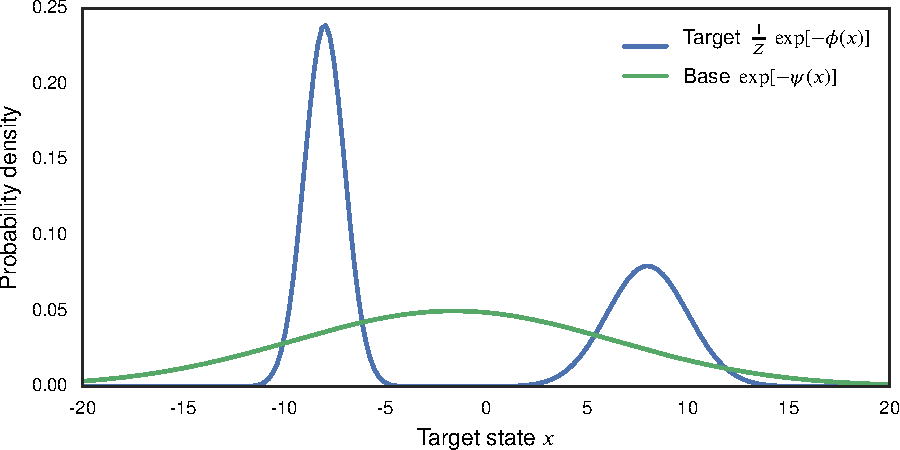
\includegraphics[width=0.95\textwidth]{images/continuous-tempering/bimodal-gm-target-and-gaussian-base} 
\caption{Target (blue curve) \& base (green curve) density functions.}\label{sfig:bimodal-gm-target-and-gaussian-base}
\end{subfigure}%
\begin{subfigure}[b]{.5\linewidth}
\vskip 0pt
\centering
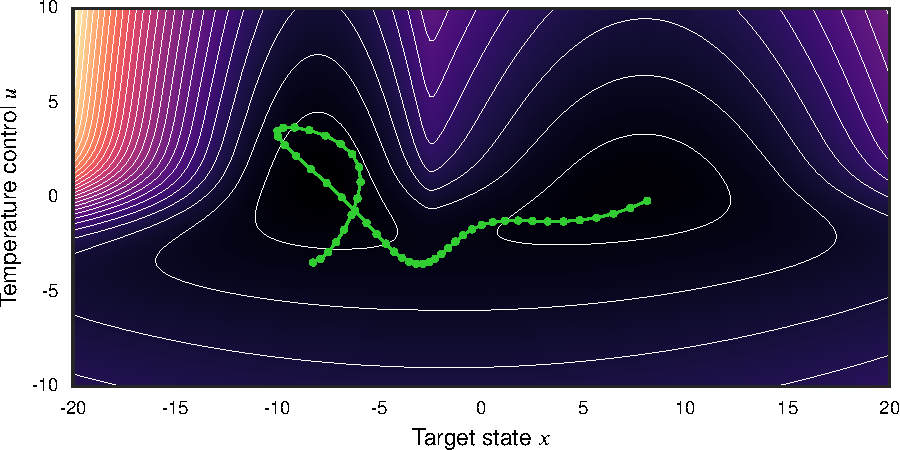
\includegraphics[width=0.95\textwidth]{images/continuous-tempering/jct-energy-and-trajectory} 
\caption{Joint energy (contour plot) \& example trajectory (green curve).}\label{sfig:jct-energy-and-trajectory}
\end{subfigure}%
\\
\begin{subfigure}[b]{.5\linewidth}
\vskip 5pt
\centering
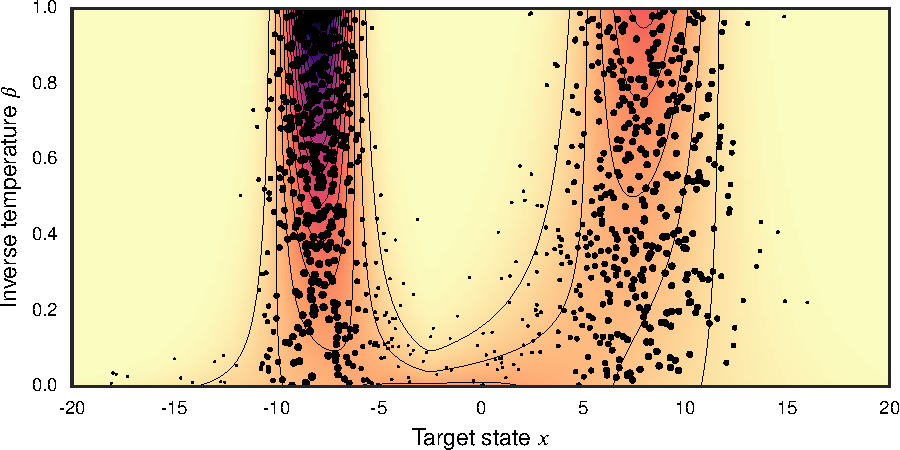
\includegraphics[width=0.95\textwidth]{images/continuous-tempering/jct-prob-dens-and-joint-samples}
\caption{Joint density (contour plot) and CT HMC samples (circles).}\label{sfig:jct-prob-dens-and-joint-samples}
\end{subfigure}
\begin{subfigure}[b]{.5\linewidth}
\vskip 5pt
\centering
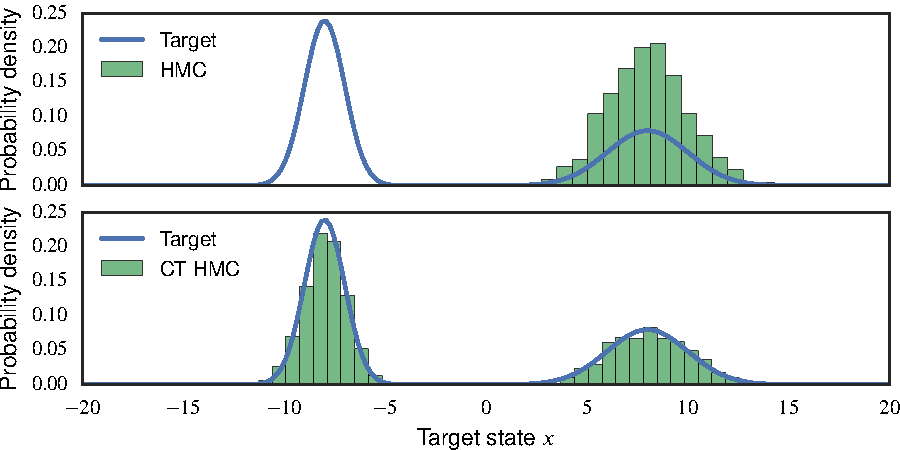
\includegraphics[width=0.95\textwidth]{images/continuous-tempering/jct-and-hmc-target-histograms}
\caption{Histograms from HMC (top) and CT HMC (bottom) samples.}\label{sfig:jct-and-hmc-target-histograms}
\end{subfigure}
\caption{Visualisations of \ac{CT} in a bimodal univariate target density. \subref{sfig:bimodal-gm-target-and-gaussian-base} A two-component Gaussian mixture target density (blue curve) and Gaussian base density (green curve) with mean and variance matched to the target. \subref{sfig:jct-energy-and-trajectory} The extended potential energy on the target state $\rvar{x}$ and temperature control variable $\rvar{u}$ (contour plot - dark colours indicate low energy) and an example simulated Hamiltonian trajectory in the joint space (green curve). The temperature control variable bridges the base and target densities lowering energy barriers in the target space. \subref{sfig:jct-prob-dens-and-joint-samples} Joint density on the target state $\rvar{x}$ and inverse temperature $\upbeta$ \eqref{eq:x-beta-joint-density} (contour plot, dark colours indicate high density) and samples from a \ac{CT} \ac{HMC} chain run in the joint space (circles, size of each circle is proportional to $\pden{\upbeta|\rvar{x}}(1\gvn x)$ and so larger symbols indicate a greater weighting in estimates of expectations with respect to the target \eqref{eq:ct-target-expc-estimator}). \subref{sfig:jct-and-hmc-target-histograms} Example target state sample histograms from running standard \ac{HMC} in the original target density (top) and running \ac{HMC} in the extended joint space (bottom).
}
\label{fig:1d-gm-vis}
\end{figure}

We give here an illustrative example of the gains of the proposed approach over standard \ac{HMC} in target densities with isolated modes. We use a one-dimensional Gaussian mixture density with two separated Gaussian components as the target density, shown by the blue curve in Figure \ref{sfig:bimodal-gm-target-and-gaussian-base}. Although performance in this toy univariate model is not necessarily reflective of that in more realistic higher-dimensional models, it has the advantage of allowing the joint density on $\rvar{x}$ and  $\upbeta = \beta(\rvar{u})$ to be directly visualised.

For the base density $\exp[-\psi(x)]$ we use a univariate Gaussian with mean and variance matched to those of the target density (corresponding to the Gaussian density minimising the \ac{KL} divergence from the target to base distribution), shown by the green curve in Figure \ref{sfig:bimodal-gm-target-and-gaussian-base}. We also set $\log \zeta = \log Z$ and so the performance here represents a `best-case' scenario for the continuous tempering approach.

The resulting potential energy ($-\log\pden{\rvar{x},\,\rvar{u}}$) on the extended $(\rvar{x},\,\rvar{u})$ space is shown in Figure \ref{sfig:jct-energy-and-trajectory}. For positive temperature control values (and so inverse temperature values close to 1), the energy surface tends increasingly to the double-well potential corresponding to the target distribution, with a high energy barrier between the two modes. For negative temperature control values the energy surface tends towards the single quadratic well corresponding to the Gaussian base density. The resulting joint energy surface allows for paths between the values of the target state $\rvar{x}$ corresponding to the two modes which have much lower potential energy barriers than the potential barrier between the two modes in the original target space, allowing simulated Hamiltonian trajectories such as that shown in green to more easily explore the target state space. 

Samples from a \ac{HMC} chain on the extended joint space are shown in Figure \ref{sfig:jct-prob-dens-and-joint-samples}, with the joint density on $(\rvar{x},\,\upbeta)$ \eqref{eq:x-beta-joint-density} shown in the background as a contoured heat map. It can be seen that the Hamiltonian dynamic is able to explore the joint space well with good coverage of all of the high density regions. The size of the points in \ref{sfig:jct-prob-dens-and-joint-samples} is proportional to $w_1(x) = \pden{\upbeta|\rvar{x}}(1\gvn x)$ and so reflects the importance weights of the samples in the estimator for expectations with respect to the target in \eqref{eq:ct-target-expc-estimator}. Importantly even points for which $\upbeta$ is close to zero can contribute significantly to the expectations if the corresponding $\rvar{x}$ value is probable under the target: this is in contrast to the extended Hamiltonian approach of \citep{gobbo2015extended} where only a subset of points corresponding to $\upbeta=1$ are used to compute expectations.

The final panel, Figure \ref{sfig:jct-and-hmc-target-histograms} shows empirical histograms on the target variable $\rvar{x}$ estimated from samples of a chain on the extended space (joint continuous tempering, bottom) and standard \ac{HMC} on the original target space (top). As can be seen the standard \ac{HMC} approach gets stuck in one mode thus does not assign any mass to the other mode in the histogram, unlike the tempered chain which identifies both modes and accurately estimates their relative masses.

\subsection{Boltzmann machine relaxations}\label{subsec:exp-bm-relaxations}

\begin{figure}[t]
\centering
\begin{subfigure}[b]{.33\linewidth}
\vskip 0pt
\centering
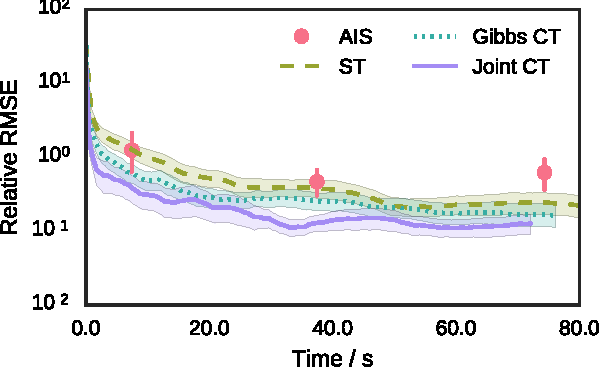
\includegraphics[width=0.95\textwidth]{images/continuous-tempering/gaussian-bm-relaxation-30-unit-scale-6-log-norm-rmses-t2} 
\caption{$\log \normconst$}\label{sfig:bmr-30-unit-scale-6-log-norm}
\end{subfigure}%
\begin{subfigure}[b]{.33\linewidth}
\vskip 0pt
\centering
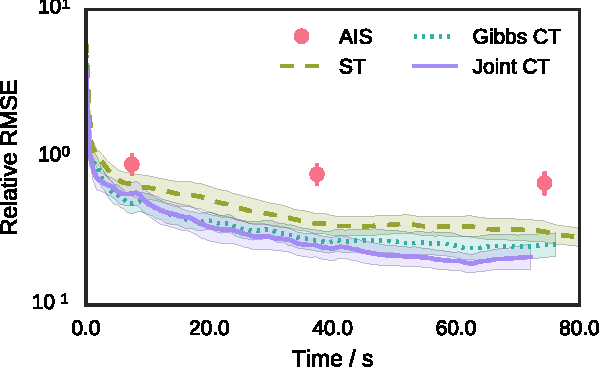
\includegraphics[width=0.95\textwidth]{images/continuous-tempering/gaussian-bm-relaxation-30-unit-scale-6-mean-rmses-t2}
\caption{$\expc{\rvct{x}}$}\label{sfig:bmr-30-unit-scale-6-mean}
\end{subfigure}
\begin{subfigure}[b]{.33\linewidth}
\vskip 0pt
\centering
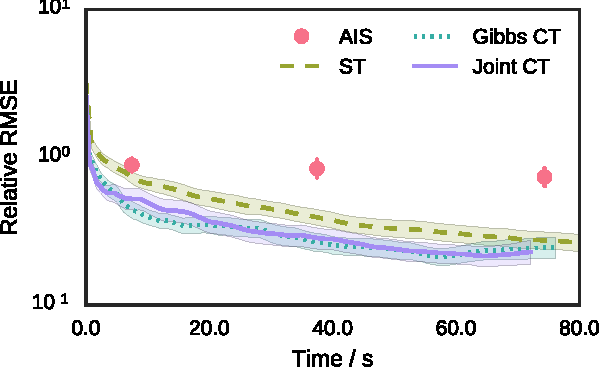
\includegraphics[width=0.95\textwidth]{images/continuous-tempering/gaussian-bm-relaxation-30-unit-scale-6-covariance-rmses-t2} 
\caption{$\expc{\rvct{x}\rvct{x}\tr} - \expc{\rvct{x}}\expc{\rvct{x}}\tr$}\label{sfig:bmr-30-unit-scale-6-covar}
\end{subfigure}
\caption[Boltzmann machine relaxation results.]{\acp{RMSE} in empirical moments estimated from \ac{MCMC} samples against run time for various thermodynamic ensemble \ac{MCMC} methods run on Gaussian Boltzmann machine relaxation target distributions. All RMSEs are relative to the RMSE of the corresponding approximate moments calculated using the moment-matched variational mixtures, so values below $1$ represent improvement on deterministic approximation. For \ac{AIS} points across time axis represent increasing number of inverse temperatures: $(1,\, 5,\,10)\times 10^3$. For \ac{ST}, Gibbs \ac{CT} and joint \ac{CT} curves show RMSEs for expectations calculated with increasing number of samples from chains. All curves / points show mean across 10 runs for each of 10 generated parameter sets. Filled regions / error bars show $\pm 3$ standard errors of mean.}
\label{fig:bmr-30-unit-scale-6-results}
\end{figure}

As a first experiment we performed inference in Gaussian mixture relaxations of a set of ten synthetic Boltzmann machine distributions \citep{zhang2012continuous}. The parameters of the Boltzmann machine distributions were randomly generated so that the corresponding relaxations are highly multimodal and so challenging to explore well. A 2D projection of samples from one generated distribution illustrating this multimodality is shown in Figure \ref{fig:bmr-samples-2d} in Appendix \ref{app:boltzmann-machine-relaxation}.

The moments of the relaxation distributions can be calculated from the moments of the original discrete Boltzmann machine distribution, which for models with a small number of binary units $D_B$ (30 in our experiments) can be computed exactly by exhaustive iteration across the $2^{D_B}$ discrete states. This allows ground truth moments to be calculated against which convergence can be checked. The parametrisation used is described in in Appendix B. A Gaussian base density and approximate normalising constant $\zeta$ was fit to each the 10 relaxation target densities by matching moments to a mixture of variational Gaussian approximations (individually fitted using a mean-field approach based on the underlying Boltzmann machine distribution) as described in section \ref{sec:choosing-base-density}.

Plots showing the \ac{RMSE} in estimates of $\log Z$ and the mean and covariance of the relaxation distribution against computational run time for different sampling methods are shown in Figure \ref{fig:bmr-30-unit-scale-6-results}. The \ac{RMSE} values are normalised by the \ac{RMSE}s of the corresponding estimated moments used in the base density (and $\log\zeta$) such that values below unity indicate an improvement in accuracy over the variational approximation. The curves shown are \ac{RMSE}s averaged over 10 independent runs for each of the 10 generated parameter sets, with the filled regions indicating $\pm 3$ standard errors of the mean. The free parameters of all methods were tuned on one parameter set and these values then fixed across all runs. All methods used a shared Theano \citep{theano2016theano} implementation running on a Intel Core i5-2400 quad-core CPU for the \ac{HMC} updates and so run times are roughly comparable.

For \ac{ST}, \emph{Rao Blackwellised} estimators were used as described in \citep{carlson2016partition}, with \ac{HMC}-based updates of the target state $\rvct{x} \gvn \upbeta$ interleaved with independent sampling of $\upbeta \gvn \rvct{x}$, and 1000 $\beta_n$ values used. For \ac{AIS}, \ac{HMC} updates were used for the transition operators and separate runs with 1000, 5000 and 10000 $\beta_n$ values used to obtain estimates at different run times. For the tempering approaches run times correspond to increasing numbers of \ac{MCMC} samples.

The two \ac{CT} approaches, Gibbs \ac{CT} and joint \ac{CT}, both dominate in terms of having lower average \ac{RMSEs} in all three moment estimates across all run times, with joint \ac{CT} showing marginally better performance on estimates of $\log\normconst$ and $\expc{\rvct{x}}$. The tempering approaches seem to outperform \ac{AIS} here, possibly as the highly multimodal nature of the target densities favours the ability of tempered dynamics to move the inverse temperature both up and down and so in and out of modes in the target density, unlike \ac{AIS} where the fixed temperature updates are more likely to end up with chains confined to a single mode after the initial transitions for low $\beta_n$.

\subsection{Hierarchical regression model}\label{subsec:exp-hier-regression}

\begin{figure}[h]
\centering
\includetikz{radon-hierarchical-linear-regression-factor-graph}
\caption{Radon hierarchical regression model.}
\label{sfig:hier-lin-regression-factor}
\end{figure}%

\begin{figure}[h]
\centering
\vskip 0pt
\centering
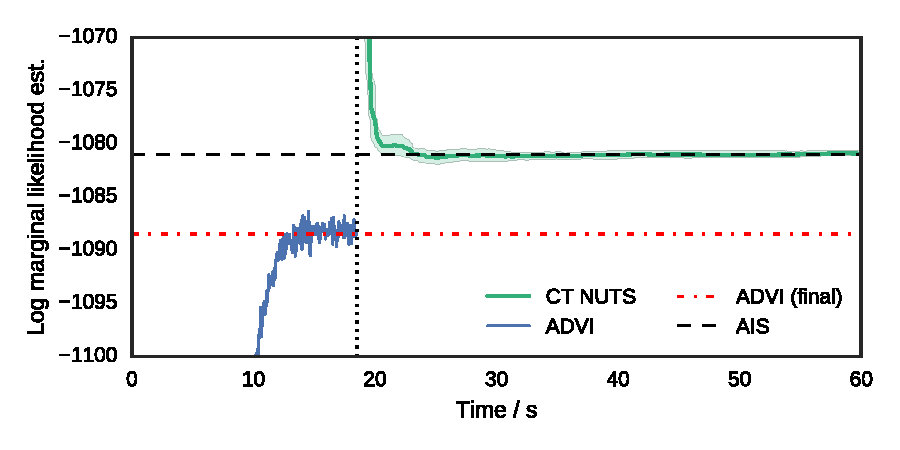
\includegraphics[width=0.8\textwidth]{images/continuous-tempering/hier-lin-regression-marg-lik-t2}
\vskip 0pt
\caption[Radon model marginal likelihood estimates.]{Log marginal likelihood estimates against run time for hierarchical regression model. Black dashed line shows estimated log marginal likelihood from a long \ac{AIS} run which is used as a proxy ground truth. The noisy blue curve shows the \emph{evidence lower bound} \ac{ADVI} objective over training and the red dot-dashed line the final converged value used for $\log\zeta$. The green curve shows log marginal likelihood estimates using samples from \ac{NUTS} chains running on the extended joint density in the estimator \eqref{eq:ct-norm-const-estimator}, with the run time corresponding to increasing samples being included in the estimator (offset by initial \ac{ADVI} run time). Curve shows mean over 10 runs and filled region $\pm 3$ standard errors of mean.}
\label{fig:hier-lin-regression}
\end{figure}

As a second experiment, we apply our joint continuous tempering approach to perform Bayesian inference in a hierarchical regression model for predicting indoor radon measurements \citep{gelman2006data}. To illustrate the ease of integrating our approach in existing \ac{HMC}-based inference software, this experiment was performed with the Python package PyMC3 \citep{salvatier2016probabilistic}, with its \ac{ADVI} feature used to fit the base density and its implementation of the adaptive
\ac{NUTS} \citep{hoffman2014no} \ac{HMC} variant used to sample from the extended space.

The regression target in the dataset is measurements of the amount of radon gas $\rvar{y}^{(i)}$ in $N=919$ households. Two continuous regressors $\vct{x}^{(i)}$ and one categorical regressor $c^{(i)}$ are provided per household. A multilevel regression model defined by the factor graph in \ref{sfig:hier-lin-regression-factor} was used. The model includes five scalar parameters $(\upsigma_{\rvct{a}},\,\upmu_{\rvct{a}},\,\upsigma_{\rvct{b}},\,\upmu_{\rvct{b}},\,\upepsilon)$, an 85-dimensional intercept vector $\rvct{a}$ and a two-dimensional regressor coefficients vector $\rvct{b}$, giving 92 parameters in total. As an example task, we consider inferring the marginal likelihood of the data under the model. Estimation of the marginal likelihood from \ac{MCMC} samples of the target density alone is non-trivial, with approaches such as the harmonic mean estimator having high variance. Here we try to establish if our approach can be used in a black-box fashion to compute a reasonable estimate of the marginal likelihood.

As our `ground truth' we use a large batch of long \ac{AIS} runs (average across 100 runs of 10000 inverse temperatures) on a separate Theano implementation of the model. We use \ac{ADVI} to fit a diagonal covariance Gaussian variational approximation to the target density and use this as the base density. \ac{NUTS} chains, initialised at samples from the base density, were then run on the extended space for 2500 iterations. The samples from these chain were used to compute estimates of the normalising constant (marginal likelihood) using the estimator \eqref{eq:ct-norm-const-estimator}. The results are shown in Figure \ref{fig:hier-lin-regression}. It can be seen that estimates from the \ac{NUTS} chains in the extended continuously tempered space quickly converge to a marginal likelihood estimate very close to the \ac{AIS} estimate, and significantly improve over the final lower bound on the marginal likelihood that \ac{ADVI} converges to.

\subsection{Generative image models}\label{subsec:exp-iwae}

\begin{figure}[h]
\centering
\begin{subfigure}[t]{\linewidth}
\vskip 0pt
\centering
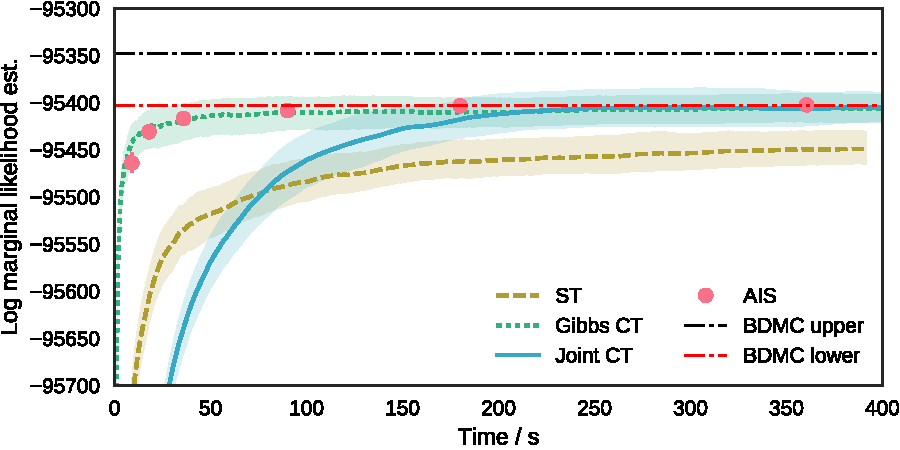
\includegraphics[width=0.95\textwidth]{images/continuous-tempering/mnist-marginal-likelihood-est-t2}
\caption{MNIST log marginal likelihood estimates.}\label{sfig:mnist-log-marg-lik}
\end{subfigure}%

\begin{subfigure}[t]{\linewidth}
\vskip 0pt
\centering
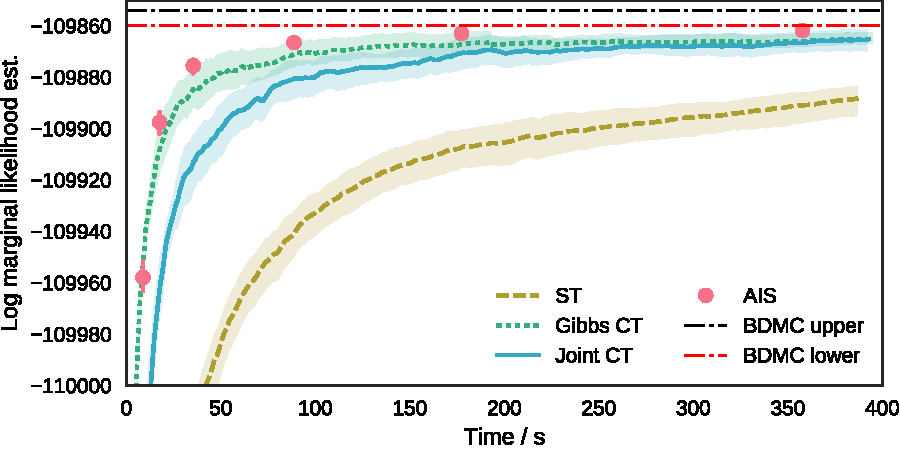
\includegraphics[width=0.95\textwidth]{images/continuous-tempering/omni-marginal-likelihood-est-t2}
\caption{Omniglot log marginal likelihood estimates.}\label{sfig:omni-log-marg-lik}
\vskip 0pt
\end{subfigure}
\caption[\acs{IWAE} marginal likelihood estimates.]{Estimates of the log joint marginal likelihood of 1000 generated images under the Bernoulli decoder distributions of two \ac{IWAE} models trained on the MNIST and Omniglot datasets against computation time. The black / red dashed lines show stochastic upper / lower bounds calculated using long \ac{BDMC} runs. For \ac{AIS} points across time axis represent increasing number of inverse temperatures: $(50,\,100,\,200,\,500,\,1000,\,2000)$. For \ac{ST}, Gibbs \ac{CT} and joint \ac{CT} curves show estimates calculated with an increasing number of samples from chains. All curves / points show mean across 10 runs. Filled regions / error bars show $\pm 3$ standard errors of mean.
}
\label{fig:iwae-marginal-likelihood-results}
\end{figure}

For our final experiments, we compared the efficiency of our \ac{CT} approaches to \ac{ST} and \ac{AIS} for marginal likelihood estimation in decoder-based generative models for images. Use of \ac{AIS} in this context was recently proposed in \citep{wu2016quantitative}. Specifically we estimate the joint marginal likelihood of 1000 generated binary images under the Bernoulli decoder distribution of two \ac{IWAE} \citep{burda2016importance} models. Each \ac{IWAE} has one stochastic hidden layer and a 50-dimensional latent space, with the two models trained on binarised versions of the MNIST \citep{lecun1998gradient} and Omniglot \citep{lake2015human} datasets using the code at \url{https://github.com/yburda/iwae}. The generated images used are shown in Appendix \ref{app:iwae-test-images}.

By performing inference on the per-image posterior densities on the latent representation given image, the joint marginal likelihood of the images can be estimated as the product of estimates of the normalising constants of the individual posterior densities. The use of generated images allows \ac{BDMC} \citep{grosse2015sandwiching} to be used to `sandwich' the marginal likelihood with stochastic upper and lower bounds formed with long forward and backward \ac{AIS} runs (averages over 16 independent runs with 10000 inverse temperatures as used in \citep{wu2016quantitative}). 

As the per-image latent representations are conditionally independent given the images, chains on all the posterior densities can be run in parallel, with the experiments in this section run on a NVIDIA Tesla K40 GPU to exploit this inherent parallelism. The encoder of the trained \ac{IWAE} models is an inference network which outputs the mean and diagonal covariance of a Gaussian variational approximation to the posterior density on the latent representation given an image and so was used to define per-image Gaussian base densities as suggested in \citep{wu2016quantitative}. Similarly the per-image $\log \zeta$ values were set using importance-weighted variational lower bound estimates for the per-image marginal likelihoods.

The results are shown in Figure \ref{fig:iwae-marginal-likelihood-results}, with the curves / points showing average results across 10 independent runs and filled regions / bars $\pm 3$ standard error of means for the estimates. Here Gibbs \ac{CT} and \ac{AIS} perform similarly, with joint \ac{CT} converging less quickly and simulated tempering significantly less efficient. The quick convergence of \ac{AIS} and Gibbs \ac{CT} here suggests the posterior densities are relatively easy for the dynamics to explore and well matched by the Gaussian base densities, limiting the gains from any more coherent exploration of the extended space by the joint \ac{CT} updates. The higher per-leapfrog-step costs of the \ac{HMC} updates in the extended space therefore mean the joint \ac{CT} approach is less efficient overall here. The poorer performance of simulated tempering here is in part due to the generation of the discrete random indices becoming a bottleneck in the \ac{GPU} implementation.

A possible reason for the better relative performance of \ac{AIS} here compared to the experiments in Section \ref{subsec:exp-bm-relaxations} is its more effective utilisation of the parallel compute cores available when running for example on a \ac{GPU}. Multiple \ac{AIS} chains can be run for each data point and then the resulting unbiased estimates for each data points marginal likelihood averaged (reducing the per data point variance) before taking their product for the joint marginal likelihood estimate. While it is also possible to run multiple tempered chains per data point and similarly combine the estimates, empirically we found that greater gains in estimation accuracy came from running a single longer chain rather than multiple shorter chains of total length equivalent to the longer chain. This can be explained by the initial \emph{warm up} transients of each shorter chain having a greater biasing effect on the overall estimate compared to running longer chains. Therefore an increase in the number of parallel compute cores available seems to give greater gains for \ac{AIS} versus the tempering methods.

\section{Discussion}

The approach we have presented is a simple but powerful extension to existing tempering methods which can both help exploration of distributions with multiple isolated modes and allow estimation of the normalisation constant of the target distribution. A key advantage of the joint \ac{CT} method is its ease of implementation - it simply requires running \ac{HMC} in an extended state space and so can easily be used for example within existing probabilistic programming software such as PyMC3 \citep{salvatier2016probabilistic} and Stan \citep{carpenter2016stan}. By updating the temperature jointly with the original target state, it is also possible to leverage adaptive \ac{HMC} variants such as \ac{NUTS} \citep{hoffman2014no} to perform tempered inference in a `black-box' manner without the need to separately tune the updates of the inverse temperature variable.

The Gibbs \ac{CT} method also provides a relatively black-box framework for tempering. Compared to \ac{ST} it removes the need to choose the number and spacing of discrete inverse temperatures and also replaces generation of a discrete random variate from a categorical distribution when updating $\upbeta$ given $\rvct{x}$ (which as seen in Section \ref{subsec:exp-iwae} can become a computational bottleneck) with generation of a truncated exponential variate (which can be performed efficiently by inverse transform sampling). Compared to the joint \ac{CT} approach, the Gibbs approach is less simple to integrate in to existing \ac{HMC} code due to the separate $\upbeta$ updates, but eliminates the need to tune the temperature control mass value $m$ and achieved similar or better sampling efficiency in the experiments in Section \ref{sec:experiments}.

Our proposal to use variational approximations within an \ac{MCMC} framework can be viewed within the context of several existing approaches which suggest combining variational and \ac{MCMC} inference methods. \emph{Variational MCMC} \citep{de2001variational} proposes using a variational approximation as the basis for a proposal distribution in a Metropolis-Hastings \ac{MCMC} method. \emph{MCMC and Variational Inference: Bridging the Gap} \citep{salimans2015markov} includes parametrised \ac{MCMC} transitions within a (stochastic) variational approximation and optimises the variational bound over these (and a base distribution's) parameters. Here we exploit cheap (relative to running a long \ac{MCMC} chain) but biased variational approximations to a target distribution and its normalising constant, and propose using them within an \ac{MCMC} method which gives asymptotically exact results to help improve sampling efficiency.